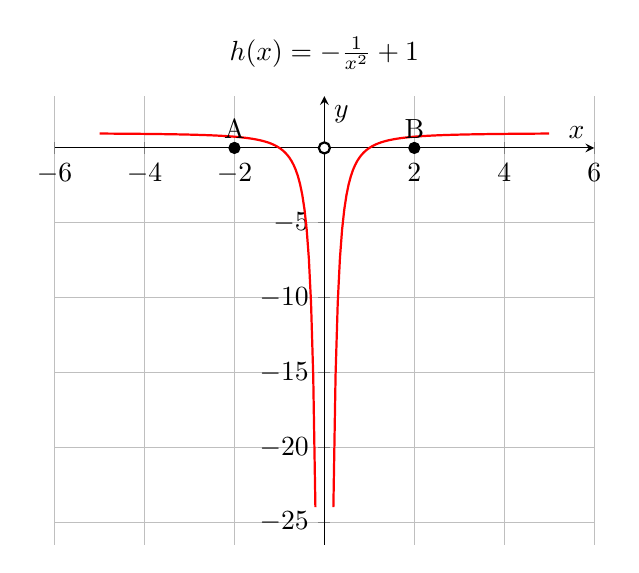
\begin{tikzpicture}
    \begin{axis}[
        axis lines = middle,
        grid = major,
        enlargelimits = true,
        xlabel={$x$},
        ylabel={$y$},
        title={$h(x) = -\frac{1}{x^2} + 1$}
    ]
    
    % Función racional
    \addplot[domain=-5:-0.2, samples=100, thick, red] {-((1)/(x^(2)))+1};
    \addplot[domain=0.2:5, samples=100, thick, red] {-((1)/(x^(2)))+1};
    
    % Puntos marcados
    \addplot[only marks, mark=*, mark options={black}, nodes near coords={A}] coordinates {(-2,0)};
    \addplot[only marks, mark=*, mark options={black}, nodes near coords={B}] coordinates {(2,0)};
    \addplot[only marks, mark=*, mark options={white}, scale=1.5] coordinates {(0,0)};
    \addplot[only marks, mark=o, mark options={black}, scale=1.5, thick] coordinates {(0,0)};
    
    \end{axis}
\end{tikzpicture}